\documentclass[../distribution_theory_notes.tex]{subfiles}
\begin{document}
\section{Aula 06 - 09 de Setembro, 2024}
\subsection{Motivações}
\begin{itemize}
 \item Continuando Topologia Fraca-*; 
 \item Regra de Leibniz;
 \item Limite Indutivo de Espaços Localmente Convexos. 
\end{itemize}
\subsection{Continuando Topologia Fraca-*}
Dando continuidade ao estudo da topologia fraca-*, descreveremos ela para o caso de E ser um TVS qualquer:

\begin{def*}
  Seja \((E, \tau )\) um TVS. Seu \textbf{dual topológico} é o conjunto \(E'\) formado por todos os funcionais lineares contínuos \(u:E\rightarrow \mathbb{C}\), onde \(\mathbb{C}\) está munido da topologia usual. \(\square\)
\end{def*}

Com esta definição, fica claro que \(E'\) é um espaço vetorial munido das operações naturalmente definidas por: dados u, v em E' e \(\lambda \) complexo, 
\begin{align*}
  & \left< u+v, x \right> = \left< u, x \right> + \left< v, x \right>,\quad x\in E\\ 
  & \left< \lambda u, x \right> = \lambda \left< u, x \right>,\quad x\in E,
\end{align*}
bastando usar a continuidade da soma e multiplicação em \(\mathbb{C}\)\footnote{por este motivo, \(\mathbb{C}\) é um TVS sobre si mesmo, constituindo um chamado \textit{corpo topológico}.}.

\begin{def*}
  Se \((E, \tau )\) é um TVS e x é um ponto de E, a \textbf{topologia fraca-* sobre E} é a topologia gerada pela família separante de seminormas dadas por 
 \begin{align*}
   p_x:&E'\rightarrow \mathbb{C}\\ 
       &u\mapsto p_x(u)\coloneqq |\left< u, x \right>|.\quad \square
 \end{align*} 
\end{def*}
  Com esta topologia, \(E'\subseteq \mathcal{F}(E; \mathbb{C})\), de modo que sua convergência fraca-* é descrita por: 
    \[
      u_{n}\substack{* \\ \longrightarrow \\ }u \Longleftrightarrow  \left< u_{n}, x \right>\substack{ \\ \longrightarrow \\ n\to \infty}\left< u, x \right>,\quad \forall x\in E,
    \]
    ou seja, se os produtos internos de cada membro da sequência de funcionais contínuos converge pontualmente em E. Sempre que considerarmos E como um TVS, suporemos que ele está munido da topologia fraca-*.

   \begin{def*}
     Um \textbf{espaço de Fréchet} é um TVS localmente convexo, metrizável e completo. \(\square\)
   \end{def*}

   Na definição acima, o ``completo'' é no sentido de que ``todo net \(\langle x_{\gamma } \rangle_{\gamma }\) de Cauchy converge para um vetor de E'', e pode ser provado que, quando E é métrico, ser completo e ser sequencialmente completo são equivalentes, permitindo-nos enunciar os resultados: 

 \begin{theorem*}
   O espaço \(\mathcal{C}^{\infty}(\Omega )\) é um espaço de Fréchet, onde \(\Omega \) é um aberto de \(\mathbb{R}^{n}\). 
 \end{theorem*}
\begin{crl*}
  O espaço \(\mathcal{C}_{c}^{\infty}(K )\) é um espaço de Fréchet, como subespaço fechado do anterior. 
\end{crl*}
\begin{theorem*}
   O espaço \(\mathcal{S}\) é um espaço de Fréchet.
 \end{theorem*}

     \begin{tcolorbox}[
     skin=enhanced,
     title=Observação,
     fonttitle=\bfseries,
   colframe=black,
     colbacktitle=cyan!75!white, 
     colback=cyan!15,
     colbacklower=black,
   coltitle=black,
     drop fuzzy shadow,
     %drop large lifted shadow
     ]
     Pode ser mostrado que, quando E é um espaço de Fréchet, então E' é sequencialmente completo, conforme foi dito anteriormente, pelo Teorema de Banach-Steinhauss.
     \end{tcolorbox}

    \begin{example}
     \begin{itemize}
       \item[1)] Considerando o dual topológico de \(\mathcal{C}^{\infty}(\Omega )\), \(\mathcal{E}'(\Omega )\), uma sequência \(\{u_{j}\}_{j}\) em \(\mathcal{E}'\) converge para uma u se, e somente se, 
         \[
           \left< u_{j}, \varphi  \right>\substack{ \\ \longrightarrow \\ j\to \infty} \left< u, \varphi  \right>,\quad \forall \varphi \in \mathcal{C}^{\infty}(\Omega );
         \]
         \item[2)] Conforme vimos na aula passada, \(\mathcal{S}'\) é o dual topológico do espaço das funções de decaimento rápido, \(\mathcal{S},\) é composto pelas distribuições temperadas e denotado por \(\mathcal{S}'\).
     \end{itemize}
    \end{example}

    \subsection{Limite Indutivo de Espaços Localmente Convexos}
    Dando continuidade ao nosso estudo dos TVS's, olharemos mais a fundo o ``maior'' e que mais generaliza o conceito de função, \(\mathcal{D}'(\Omega ),\) o dual de \(\mathcal{C}_{c}^{\infty}(\Omega )\) munido da topologia ``limite indutivo'', mas antes, veremos mais exemplos de aplicações lineares contínuas entre TVS's,
   \begin{lemma*}
     Sejam \(f, g\) em \(\mathcal{C}^{\infty}(\Omega )\) e \(\alpha \in \mathbb{Z}_{+}^{n}\). Então, vale a regra: 
       \[
         \partial^{\alpha }(fg)=\sum\limits_{\beta+\gamma =\alpha }^{}\frac{\alpha!}{\beta!\gamma!}(\partial^{\beta }f)(\partial^{\gamma }g).
       \]
   \end{lemma*}
   Quando \(n=1\) e \(\alpha =m\in \mathbb{Z}_{+}\), então 
     \[
       (fg)^{(m)} = \sum\limits_{k=0}^{m}\frac{m!}{k!(m-k)!}f^{(k)}g^{(m-k)}.
     \]
    \begin{lemma*}
      Se \(a\in \mathcal{C}^{\infty}(\Omega )\) e \(S:\mathcal{C}^{\infty}(\Omega )\rightarrow \mathcal{C}^{\infty}(\Omega )\) é dado por \(s\varphi\coloneqq a \varphi \), então s é linear e contínuo.
    \end{lemma*}
    
    Conforme vimos nos exemplos, uma das grandes vantagens das topologias induzidas por seminormas é que elas eliminam os problemas de descontinuidade do operador derivada; mais precisamente, neles vale o 
   \begin{theorem*}
     Seja \(\Omega \) um aberto qualquer de \(\mathbb{R}^{n}\). Não existe uma \textit{norma} em \(\mathcal{C}^{\infty}(\Omega )\) segundo a qual o operador linear 
       \[
         T=\frac{\partial^{}}{\partial x_{j}^{}}:\mathcal{C}^{\infty}(\Omega )\rightarrow \mathcal{C}^{\infty}(\Omega )
       \]
       seja contínuo, qualquer que seja \(j=1,2,\dotsc ,n.\)
   \end{theorem*}
  \begin{proof*}
    Com efeito, se \(\Vert \cdot  \Vert\) é uma norma qualquer em \(\mathcal{C}^{\infty}(\Omega )\) e, para cada \(\lambda \) complexo, considerarmos \(f_{\lambda }(x)\coloneqq e^{\lambda x_{j}}\), veremos que 
      \[
        \frac{\partial^{}f_{\lambda }}{\partial x_{j}^{}}(x)=\lambda e^{\lambda x_{j}}=\lambda f_{\lambda }(x),
      \]
      que leva à conclusão de que 
        \[
          \frac{\partial^{}f_{\lambda }}{\partial x_{j}^{}} = \lambda f_{\lambda } \Rightarrow \biggl\Vert \frac{\partial^{}f_{\lambda }}{\partial x_{j}^{}} \biggr\Vert=|\lambda |\cdot \Vert f_{\lambda } \Vert,
        \]
        ou seja, 
          \[
            \frac{\Vert Tf_{\lambda } \Vert}{\Vert f_{\lambda } \Vert}=|\lambda |.
          \]
          Portanto, 
            \[
              \sup_{f\neq 0}\frac{\Vert Tf \Vert}{\Vert f \Vert}=\infty,
            \]
            e T não pode ser limitado, uma contradição. \qedsymbol
  \end{proof*}
   \begin{tcolorbox}[
   skin=enhanced,
   title=Observação,
   fonttitle=\bfseries,
 colframe=black,
   colbacktitle=cyan!75!white, 
   colback=cyan!15,
   colbacklower=black,
 coltitle=black,
   drop fuzzy shadow,
   %drop large lifted shadow
   ]
   É claro que, na notação de multi índices, \(\partial^{\beta +\gamma }f=\partial^{\beta }(\partial^{\gamma }f)\) simplesmente compondo derivadas e usando indução; a exemplo, 
     \[
       \partial^{e_{j}+e_{k}}f = \biggl(\frac{\partial^{}}{\partial x_{j}^{}}\circ \frac{\partial^{}}{\partial x_{k}^{}}\biggr)f = \frac{\partial^{}}{\partial x_{j}^{}}\biggl(\frac{\partial^{}f}{\partial x_{k}^{}}\biggr) = \partial^{e_{j}}(\partial^{e_{k}}f).
     \]
   \end{tcolorbox}
  \begin{example}
    Para o primeiro exemplo, sejam \(\Omega \) um aberto de \(\mathbb{R}^{n}\) e \(a:\Omega \rightarrow \mathbb{C}\) uma função \(\mathcal{C}^{\infty}(\Omega )\). O operador 
   \begin{align*}
     T=a(x)\frac{\partial^{}}{\partial x_{j}^{}}:&\mathcal{C}^{\infty}(\Omega )\rightarrow \mathcal{C}^{\infty}(\Omega )\\ 
                                                 &\varphi \mapsto a(x)\frac{\partial^{}\varphi }{\partial x_{j}^{}}
   \end{align*}
   é contínuo, onde \(\mathcal{C}^{\infty}(\Omega )\) está munido d topologia dada pelas seminormas \(p_{(m, j)}.\) Com efeito, dados índices m e j naturais, e \(\varphi \) um elemento de \(\mathcal{C}^{\infty}(\Omega )\), calculamos: 
  \begin{align*}
    p_{(m, j)}(T\varphi )&=\sum\limits_{|\alpha |\leq m}^{}\sup_{x\in K_{j}} \biggl\vert \partial^{\alpha }\biggl(a \frac{\partial^{}\varphi }{\partial x_{j}^{}}\biggr)(x) \biggr\vert\\
                         &=\sum\limits_{|\alpha |\leq m}^{}\sup_{K_{j}}\bigl\vert \sum\limits_{\beta+\gamma =\alpha }^{} \frac{\alpha!}{\beta!\gamma!}(\partial^{\beta }a(x))\biggl(\partial^{\gamma }\frac{\partial^{}\varphi }{\partial x_{j}^{}}(x)\biggr)\bigr\vert\\ 
                         &\leq \sum\limits_{|\alpha |\leq m}^{}\sum\limits_{\beta +\gamma =\alpha }^{}\frac{\alpha!}{\beta!\gamma!}\sup_{K_{j}}\biggl\vert \partial^{\beta }a(x)\partial^{\gamma +e_{j}}\varphi(x) \biggr\vert\\ 
                         &\leq \sum\limits_{|\alpha |\leq m}^{}\sum\limits_{\beta +\gamma =\alpha }^{}\biggl[\frac{\alpha!}{\beta!\gamma!}\sup_{K_{j}}\bigl\vert \partial^{\beta }a(x)\bigr\vert\biggr]\biggl[\sup_{K_{j}}\bigr\vert\partial^{\gamma +e_{j}}\varphi(x) \bigr\vert\biggr]\\ 
                         &= C \sum\limits_{|\alpha |\leq m}^{} \sup_{K_{j}}\biggl\vert \partial^{\gamma +e_{j}}\varphi (x) \biggr\vert,
  \end{align*}
  onde 
    \[
      C=\sum\limits_{|\alpha |\leq m}^{}\sum\limits_{\beta +\gamma =\alpha }^{}\biggl[\frac{\alpha!}{\beta!\gamma!}\sup_{K_{j}}\bigl\vert \partial^{\beta }a(x)\bigr\vert\biggr]
    \] 
    é uma constante que depende apenas de m, j e a, não de \(\varphi \). Além disso, colocando \(\alpha '= \alpha +e_{j}\), tem-se \(|\alpha |'\leq |\alpha |+1 \leq m+1\), tal que
      \[
        \sum\limits_{|\alpha |\leq m}^{}\sup_{K_{j}}|\partial^{\gamma +e_{j}}\varphi (x)|\leq \sum\limits_{|\alpha |\leq m+1}^{}\sup_{x\in K_{j}}|\partial^{\alpha '}\varphi (x)|=p_{(m+1, j)}(\varphi ).
      \]

      Em conclusão, para todo \(\varphi \) em \(\mathcal{C}^{\infty}(\Omega )\), 
        \[
          p_{(m, j)}(T\varphi )\leq Cp_{(m+1, j)}(\varphi ),
        \]
        provando que T é contínuo.
  \end{example}
 \begin{example}
   Nas condições acima, se \(K\subseteq \Omega \) é um compacto com \(\mathrm{int}(K)\neq\emptyset\), então 
     \[
       a \frac{\partial^{}}{\partial x_{j}^{}}:\mathcal{C}_{c}^{\infty}(K)\rightarrow \mathcal{C}_{c}^{\infty}(K)
     \]
     está bem definido e é contínuo. Para isto, basta ver que \(a \frac{\partial^{}}{\partial x_{j}^{}}\) leva funções com suporte em K em funções com suporte em K, decorrente do fato de que 
       \[
         \mathrm{supp}(fg)\subseteq \mathrm{supp}(f)\cap \mathrm{supp}(g),
       \]
       tendo em vista que 
         \[
           fg(x)\neq 0 \Rightarrow f(x)\neq 0 \quad\&\quad g(x)\neq 0 \Rightarrow x\in \mathrm{supp}(f)\cap \mathrm{supp}(g).
         \]
        Como o conjunto formado pela interseção é fechado, segue a continuidade.
 \end{example}
\begin{example}
  Seja \(a\in \mathcal{C}^{\infty}(\mathbb{R}^{n})\) tal que, para cada \(\alpha \in \mathbb{Z}_{+}^{n}\), existe um natural \(m_{\alpha }\) tal que 
    \[
      \sup_{x\in \mathbb{R}^{n}}(1+|x|)^{-m_{\alpha }}|\partial^{\alpha }a(x)|<\infty;
    \]
    então, 
      \[
        T = a \frac{\partial^{}}{\partial x_{j}^{}}:\mathcal{S}\rightarrow \mathcal{S}
      \]
      está bem definido e é contínuo.
\end{example}
\begin{theorem*}
  Se \(P(x, D)=\sum\limits_{|\alpha |\leq m}^{}a_{\alpha }(x)\partial^{\alpha },\) onde, para cada \(|\alpha |\leq m\), \(a_{\alpha }\in \mathcal{C}^{\infty}(\Omega )\), então 
    \[
      P(x, D):\mathcal{C}^{\infty}(\Omega )\rightarrow \mathcal{C}^{\infty}(\Omega ) \quad\&\quad  P(x, D):\mathcal{C}_{c}^{\infty}(K )\rightarrow \mathcal{C}_{c}^{\infty}(K )
    \]
    são contínuas.
\end{theorem*}
\begin{proof*}
  Basta observar que cada 
    \[
      \partial^{\alpha }=\partial_{1}^{\alpha_{1}} \circ\partial_{2}^{\alpha_{2}} \circ\cdots\circ \partial_{n}^{\alpha_{n}}
    \]
    é a composição de aplicações contínuas. Portanto, \(Sf=a_{\alpha }f\) também é. \qedsymbol
\end{proof*}

\hypertarget{inductive_limit}{\begin{theorem*}
  Seja \((E, \tau_{j})_{j\in \mathbb{N}}\) uma sequência de TVS's localmente convexos tal que \(E_{j}\subseteq E_{j+1}\) para todo j natural. Consideremos 
 \begin{align*}
   & E \coloneqq \bigcup_{j=1}^{\infty}E_{j}; \text{ e}\\
   & \mathcal{B}\coloneqq \{x+W: W\subseteq E \text{ é convexo e equilibrado},\; W\cap E_{j}\in \tau_{j},\; \forall j\in \mathbb{N}\}.
 \end{align*}
 Valem as seguintes propriedades: 
\begin{itemize}
  \item[i)] E é um espaço vetorial; 
    \item[ii)] \(\mathcal{B}\) é base para uma topologia \(\tau \) localmente convexa em E, compatível com sua estrutura linear; 
      \item[iii)] Para todo j natural, \(E_{j}\hookrightarrow E\);
        \item[iv)] Se \(f:E\rightarrow F\) é linear e \((F,  \tau_{F})\) é um TVS localmente convexo, então f é contínua se, e somente se, \(f|_{E_{j}}:E_{j}\rightarrow F\) é contínua para todo j natural;
          \item[v)] Se existir uma norma \(p_{0}:E\rightarrow \mathbb{R}\) tal que \(p_{0}|_{E_{j}}:E_{j}\rightarrow \mathbb{R}\) é contínua para todo j natural, então \(\tau \) é Hausdorff; e
\item[v)] Se cada \(E_{j}\) é Fréchet, então E é completo.
\end{itemize}
\end{theorem*}}
\begin{figure}[H]
\begin{center}
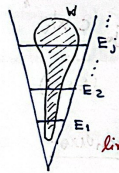
\includegraphics[height=0.5\textheight, width=0.5\textwidth, keepaspectratio]{./Images/inductive_limit_06.png}
\end{center}
\caption{visualização do limite indutivo dos \(E_{j}\)'s.}
\end{figure}

\begin{proof*}
  (i) Para este item, precisamos definir as operações deste espaço vetorial; com efeito, elas são definidas assim: dados x, y em E e \( ul\) complexo, existe j natural tal que \(x, y\in E_{j}\) e pomos: 
    \[
      x+_{E}y\coloneqq x +_{E_{j}}y \quad\&\quad \lambda \cdot_{E} x = \lambda_{E_{j}} \cdot x,
    \]
    que não dependem do j, tornando-as bem definidas e satisfazendo os axiomas de espaço vetorial. 

    (ii) Precisamos provar que \(\mathcal{B}\) satisfaz as duas condições do teorema de topologia geral que caracteriza bases. Tendo em vista que \(W=E\in \mathcal{B}\) pois E é convexo, equilibrado e satisfam 
      \[
        E\cap E_{j}=E_{j}\in \tau_{j},\quad \forall j,
      \]
      a primeira condição já segue. A segunda condição já é mais delicada: seja 
        \[
          x\in (x_1+W_{1})\cap (x_2+W_2), \quad x_1+W_1, x_2+W_2\in \mathcal{B}.
        \]
        Podemos escolher um j natural tal que \(x, x_1, x_2\in E_{j_{0}}\). Assim, por definição, 
          \[
            x-x_1\in W_1,\; x-x_2\in W_2, \;\&\; W_1\cap E_{j_{0}}, W_2\cap E_{j_{0}}\in \tau.
          \]
          Como, para \(i=1, 2,\) a aplicação 
         \begin{align*}
          m_{(x-x_{i})}:&\mathbb{C}\rightarrow E_{j_{0}}\\ 
                        &\lambda \mapsto m_{(x-x_{i})}(\lambda )=\lambda (x-x_{i})
         \end{align*}
         é contínua em \(\lambda =1\), existe \(r_{i}\) positivo tal que 
           \[
             i=1,2 \;\&\; |\lambda -1|<r_{i} \Rightarrow \lambda (x-x_{i})\in W_{i}\cap E_{j_{0}}\subseteq W_{i}.
           \]
Em particular, para \(\lambda  = 1 + r_{i}/2\), tem-se 
    \[
      x-x_{i}\in \frac{1}{1+r_{i}/2}W_{i}.
    \]
    Daí, tomando 
      \[
        \delta_{i}=\frac{1}{1+\frac{r_{i}}{2}}, 
      \]
      segue que \(\delta_{i}\in (0, 1)\) e, sendo \(W_{i}\) convexo, 
        \[
          \delta_{i} W_{i} + (1-\delta_{i})W_{i}=W_{i},
        \]
        donde 
          \[
            x-x_{i}\in \delta_{i}W_{i} \Rightarrow x\in x_{i}+\delta_{i}W_{i}\Rightarrow x+(1-\delta_{i})W_{i}\subseteq x_{i}+\delta_{i}W_{i}+(1-\delta_{i})W_{i} = x_{i}+W_{i},
          \]
          e, pondo \(W=[(1-\delta_{1})W_1]\cap [(1-\delta_2)W_2]\), obtemos que W é convexo, equilibrado, satisfaz \(W\cap E_{j}\in \tau_{j}\) para todo j, e 
            \[
              x+W\subseteq (x_1+W_1)\cap (x_2+W_2)
            \]
            (Aqui, dizemos que \(x+W\subseteq W\subseteq x+(1-\delta_{i})W_{i}\)). Por definição, cada um dos B's em \(\mathcal{B}\) é convexo. A compatibilidade de \(\tau \) com a estrutura linear é deixada de exercício.

            (iii) Se 
           \begin{align*}
             I_{j}:&(E_{j}, \tau_{j})\rightarrow (E, \tau )\\ 
                   &x\mapsto I_{j}(x)=x,
           \end{align*}
           então \(I_{j}^{-1}(W)=W\cap E_{j}\), mostrando que \(I_{j}\) é contínua, tendo em vista que \(\mathcal{B}_{0}=\{W\subseteq E:\; W\cap E_{j}\in \tau_{j}, W \text{ convexo e equilibrado}\}\) é SFV da origem de E.

           (iv) Se \(f:E\rightarrow F\) é contínua, então 
             \[
               f|_{E_{j}}=f\circ I_{j}:E_{j}\rightarrow F
             \]
             é contínua pela parte (iii). Reciprocamente, se \(\mathcal{C}\) for um SFV convexas e equilibradas da origem, então dado \(V\in \mathcal{C},\) a pré imagem \(f^{-1}(V)\) é em si um convexo equilibrado, com 
               \[
                 f^{-1}(V)\cap E_{j} = (f|_{E_{j}})^{-1}(V)\in \tau_{j},\quad \forall j.
               \]
               Portanto, \(f^{-1}(V)\in \mathcal{B}\) e f é contínua. \qedsymbol

               (v) Sob quais condições \(\tau \) seria Hausdorff? Suponhamos que exista uma norma \(p_{0}:E\rightarrow \mathbb{R}\) tal que \(p_{0}|_{E_{j}}\) é norma contínua em \(E_{j}\) para todo j;, então, \(\tau \) é Hausdorff, tendo em vista que 
                 \[
                   x\neq y,\; \frac{\delta }{2} \Rightarrow \underbrace{p^{-1}(p(x)+\delta/2)}_{W}\cap \underbrace{p^{-1}(p(y)+\delta/2)}_{V} = \emptyset,
                 \]
                 com We e V abertos, pois \(W\cap E_{j}\) e \(V\cap E_{j}\) estão em \(\tau_{j}\) pela continuidade de \(p_{0}|_{E_{j}}\) para todo j, com W e V convexos e equilibrados, portanto provando o teorema. \qedsymbol
\end{proof*}
  

\end{document}
